\chapter{Conclusions \& Extensions}
\label{sec:Conclusions}
\chaptermark{Conclusions \& Extensions}

Obtaining experimental evidence for the Higgs boson has been a major goal of the particle physics research since the conception of the LHC. Finding and characterizing this boson is key to the complete picture of electroweak symmetry breaking. This effort has been a major focus of the CMS collaboration. This thesis work focused on this search and characterization using the four-lepton final state. It offers a series of extremely important and groundbreaking measurements that were proposed an carried out on the observed data.

This thesis presents the observation of the new boson, studies of its production and decay rates, constraints on the total width, and measurements of its spin and parity properties. When the Higgs boson was discovered in 2012, it was widely believed that the study of these properties would require much more data than CMS has collected so far. Using the kinematics of the four-lepton final state in novel and efficient ways these measurements were made possible far before more conventional approaches.

All of the measurements presented here will improve with time, simply by collecting more data from the LHC data from 2015 and beyond because they are statistically limited. Additionally, many of these measurements have already been extended including information from other decay channels to say more about the observed boson. Many of these extensions were directly inspired and made possible by the work presented here, while others developed their own techniques.

\section{$H \to ZZ \to 4\ell$ Search \& Production Mechanism}
\label{sec:Summary_ProducitonDecay}

The observation of the new boson is confirmed in the $4\ell$ final state, using data from an integrated luminosity of $\unit{5.1}{\invfemtobarn}$ of proton-proton collisions at a center of mass energy of $\sqrt{s} = \unit{7}{\TeV}$, and $\unit{19.7}{\invfemtobarn}$ at $\sqrt{s} = \unit{8}{\TeV}$. The data show a local significance of
6.8 standard deviations above the expected background. Upper
limits at the 95\% C.L. exclude the SM-like Higgs boson in the mass
ranges $\unit{114.5--119.0}{\GeV}$ and $\unit{129.5--832.0}{\GeV}$, for an expected
exclusion range for the background-only hypothesis of $\unit{115--740}{\GeV}$. The production cross section of the new boson times the branching
fraction to four leptons is measured to be $\mu = 0.93^{+0.26}_{-0.23}\text{(stat.)} ^{+0.13}_{-0.09}\text{(syst.)}$ times that
predicted by the standard model ($\mu = 1$ is SM Higgs boson). Those cross sections times branching ratios associated with fermions and
vector bosons are $\mu_{ggH,t\bar{t}H} = 0.80^{+0.46}_{-0.36}$ and $\mu_{\text{VBF}, VH} = 1.7^{+2.2}_{-2.1}$, respectively,
consistent with the SM expectations ($\mu = 1$). All production and decay properties of the observed new boson in the
four-lepton final state are consistent, within their uncertainties,
with the expectations for the SM Higgs boson.
 
\subsection{Extensions}

The limits that were found using the $4\ell$ final state have been extended by combining the results with the other $H \to ZZ$ and $H \to WW$ final state results. In \cite{Khachatryan:2015cwa} a heavy Higgs boson with standard model-like couplings and decays are excluded from $\unit{145--1000}{\GeV}$ shown in figure \ref{fig:BSM_limits}. Additionally, these results are re-interpreted as a search for a heavy, narrow resonance as electroweak singlet partner of the standard model Higgs boson. No significant excess over the expected standard model background has been observed and exclusion limits have been set \cite{Khachatryan:2015cwa}. These results actually use a MELA discriminant based on the jet kinematics to separate signal from background rather than the $\mathcal{D}_{jet}$ discriminant. This discriminant takes the four-momenta of the jets produced in addition to the leptons and outputs a discriminating variable based on the matrix element calculation of VBF and $gg \to H +2\text{jets}$ \cite{Anderson:2013afp}.


\begin{figure}
\begin{center}
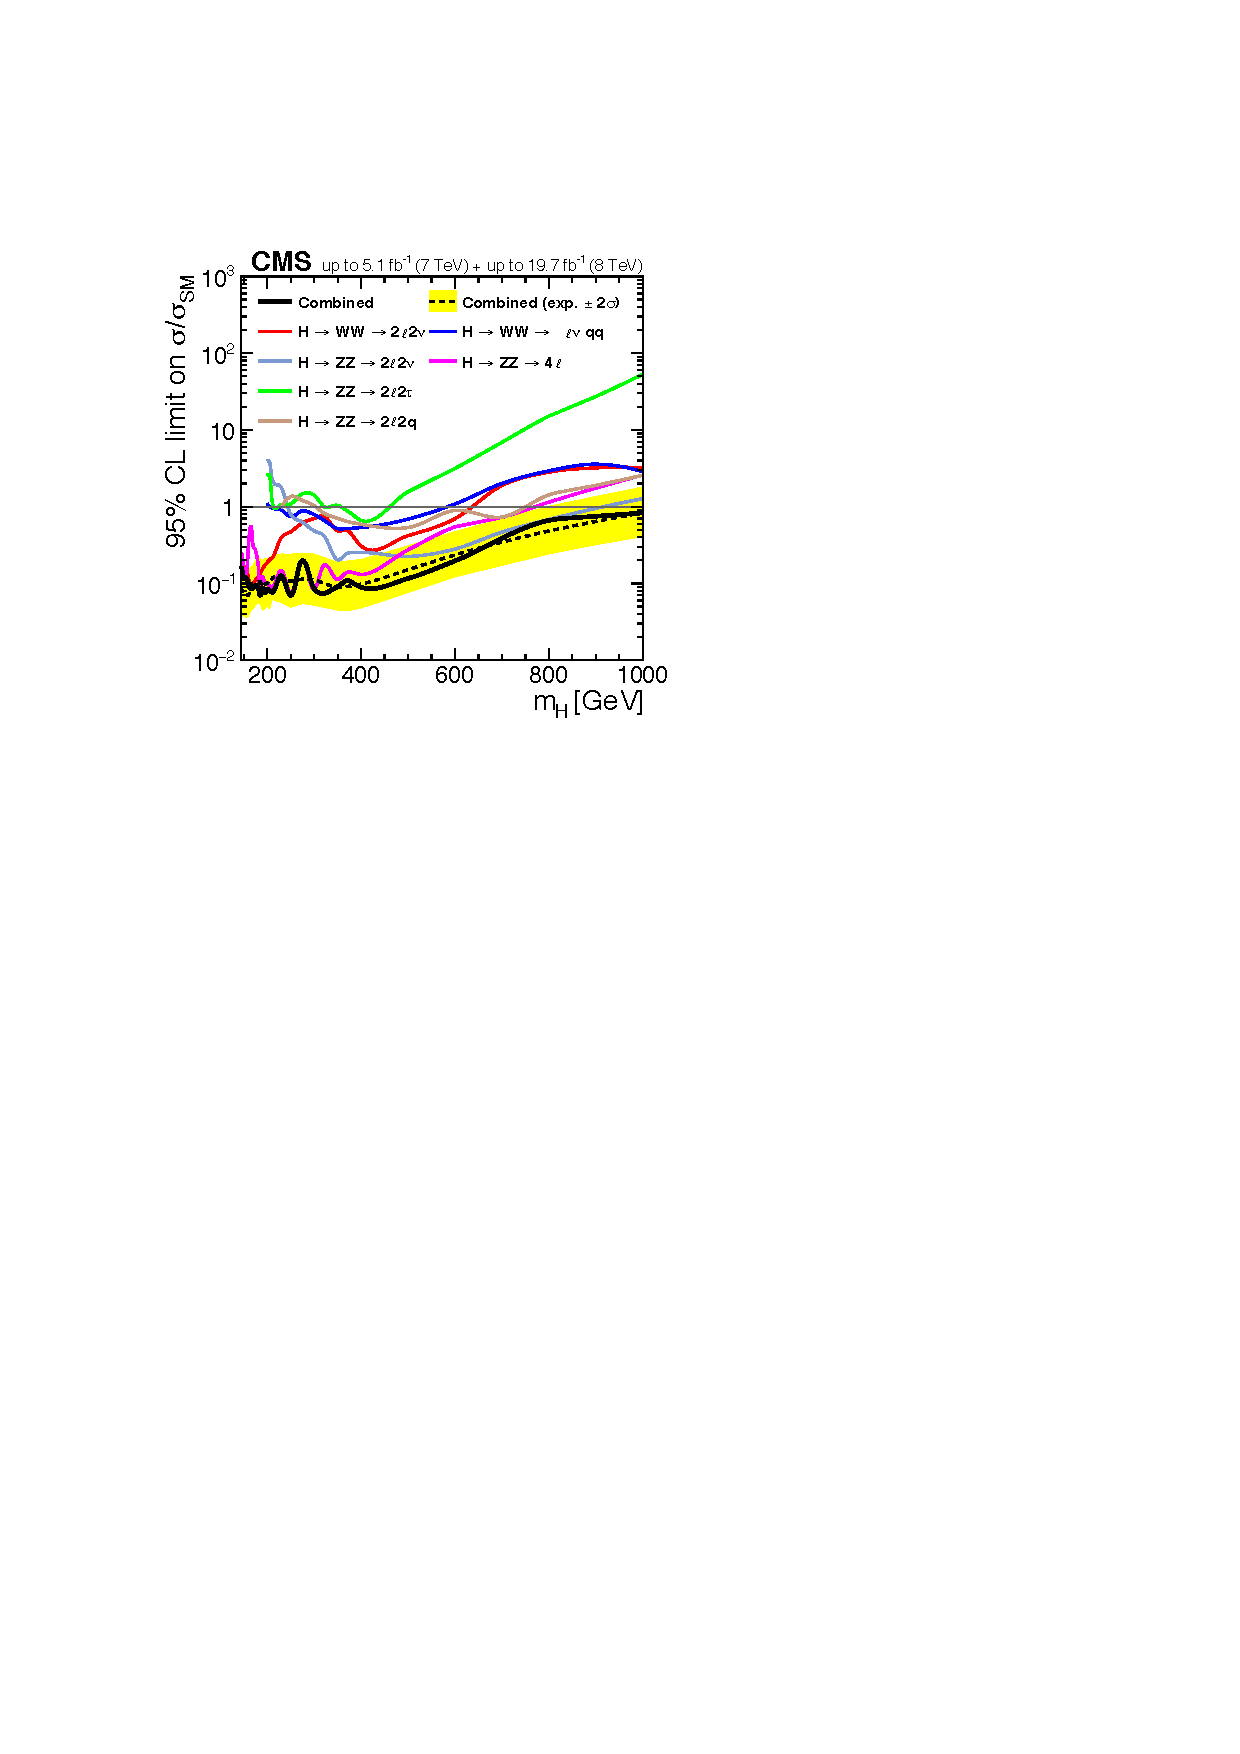
\includegraphics[width=.65\linewidth]{{Conclusion/combinedSM_def}.pdf}
\caption[Combined results of $H \to ZZ$ and $H \to WW$ in the search of a heavy, SM-like Higgs boson with SM couplings, line shape and decays. Upper limits at 95\% C.L. set for each of the contributing final states and their combination.]{Combined results of $H \to ZZ$ and $H \to WW$ in the search of a heavy, SM-like Higgs boson with SM couplings, line shape and decays. Upper limits at 95\% C.L. set for each of the contributing final states and their combination \cite{Khachatryan:2015cwa}.}
\label{fig:BSM_limits}

\end{center}
\end{figure}

The study of the production mechanisms has also been used to make a robust set of CMS results combining many different Higgs search channels. In \cite{Khachatryan:2014jba} the results from the $4\ell$ studies were combined to set extremely robust limits on the global $\mu = 1.00 \pm 0.09 \text{(stat.)} ^{+0.08}_{-0.07} \text{(theo.)} \pm 0.07 \text{(syst.)}$ (at $m_{H} = \unit{125.0}{\GeV}$) and to show the consistency of the 0/1 jet and dijet signal strengths with the other decay channels, figure \ref{fig:Comb_mu}. Similarly, the results for the production mechanism can be compared to the other final states and used to show how consistent the data from CMS is with the predicted SM Higgs boson.

\begin{figure}
\begin{center}
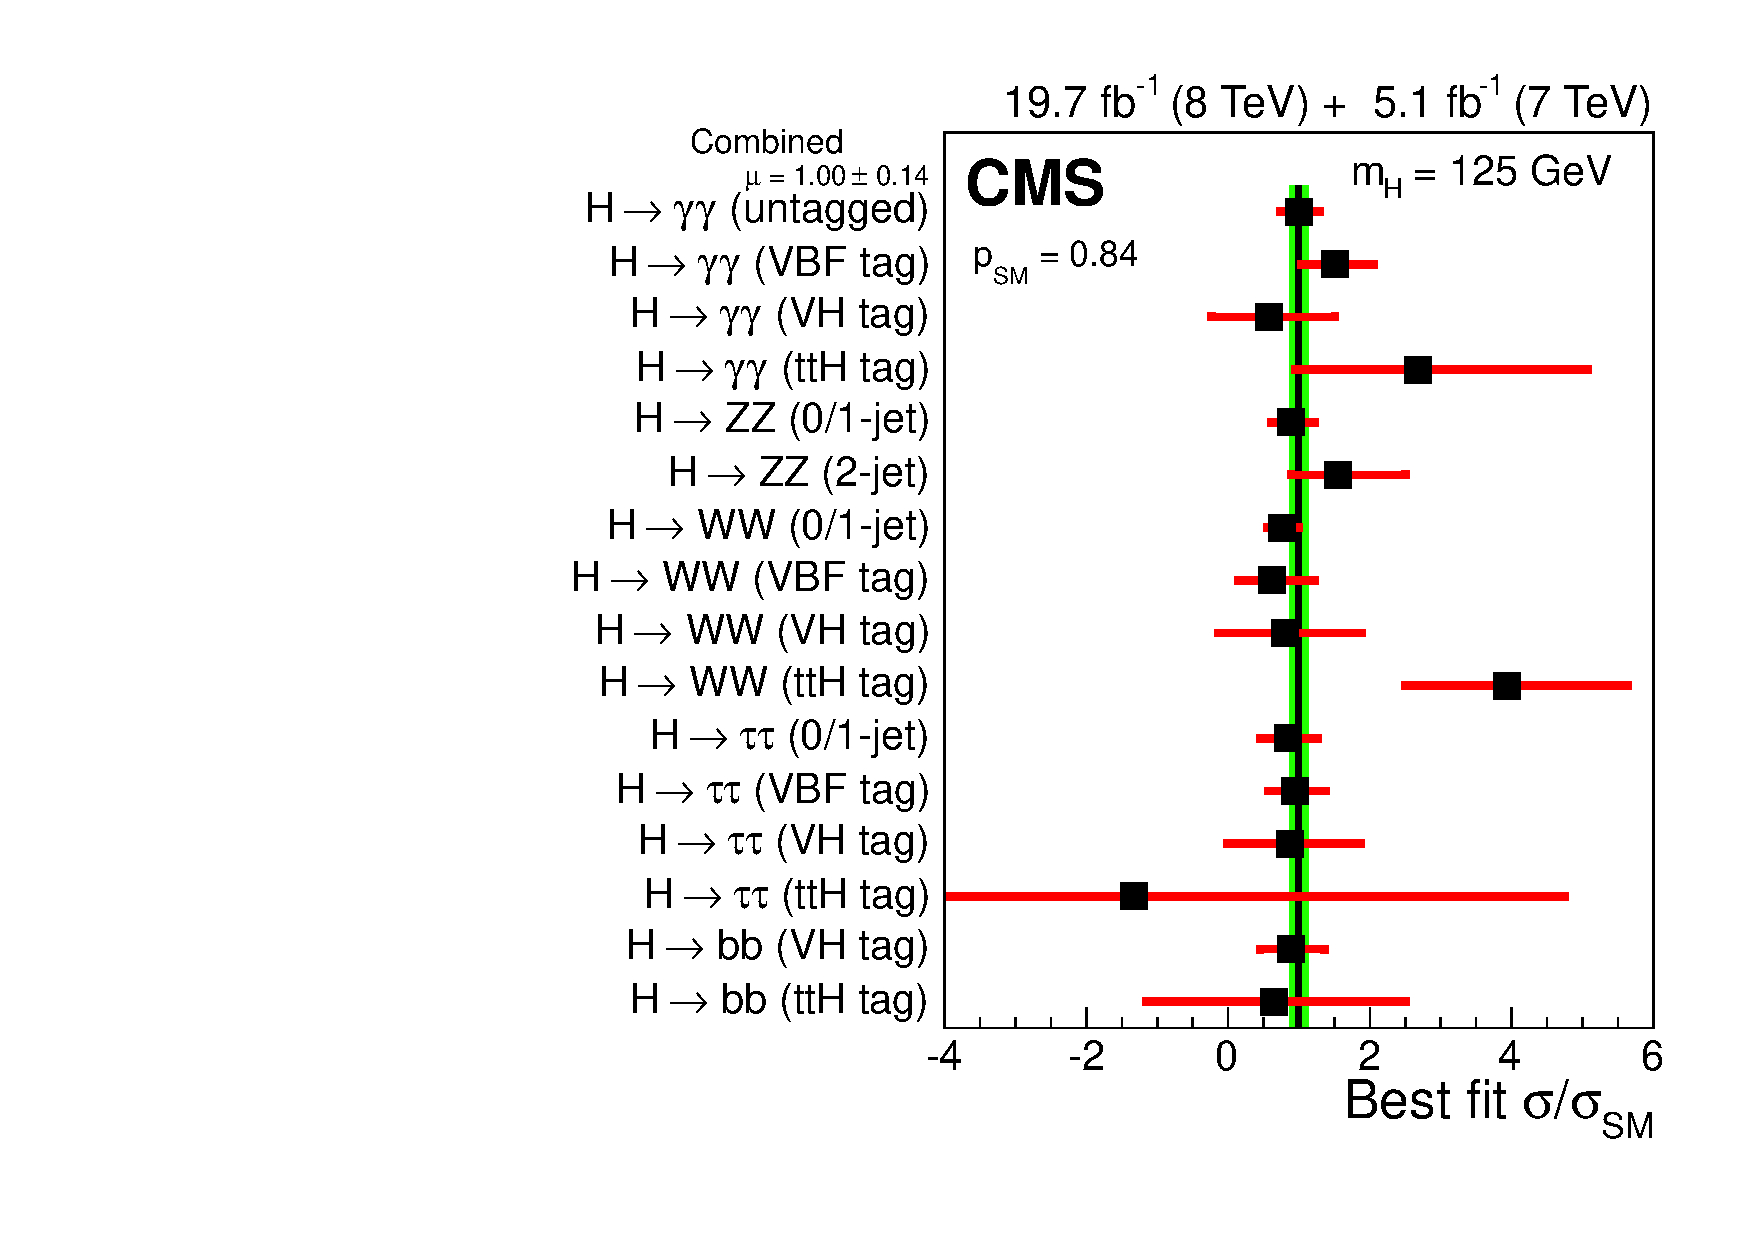
\includegraphics[width=.45\linewidth]{{Conclusion/sqr_mlz_ccc_mH125.0_16}.pdf}
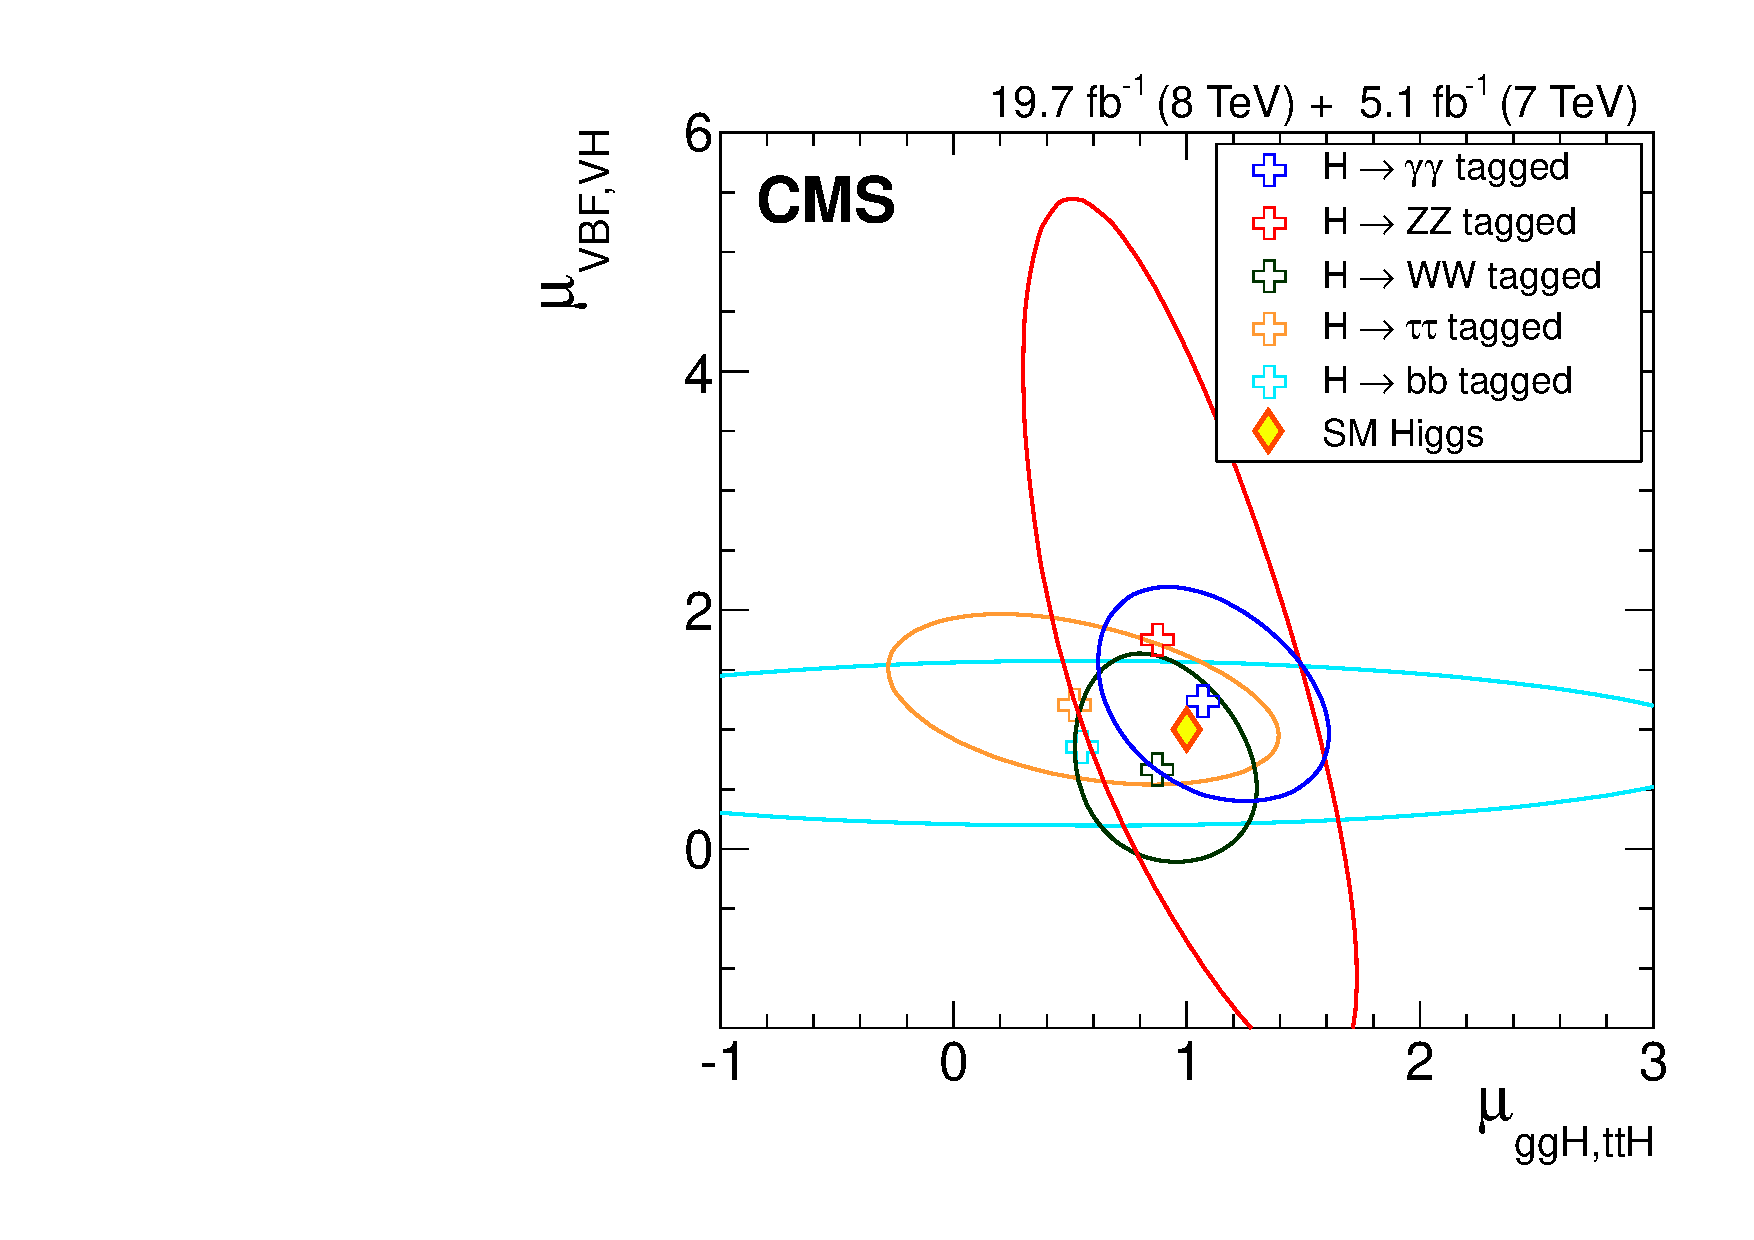
\includegraphics[width=.45\linewidth]{{Conclusion/sqr_rvrf_scan_2d_all_68}.pdf}
\caption[(left) Values of the best-fit $\sigma/\sigma_{SM}$ for the combination (solid vertical line) and for subcombinations by predominant decay mode and additional tags targeting a particular production mechanism. (right) The 68\% C.L. regions (bounded by the solid curves) for signal strength of the ggH and $t\bar{t}H$, and of the VBF and VH production mechanisms: $\mu_{ggH,t\bar{t}H}$ and $\mu_{\text{VBF}, VH}$, respectively ]{(left) Values of the best-fit $\sigma/\sigma_{SM}$ for the combination (solid vertical line) and for subcombinations by predominant decay mode and additional tags targeting a particular production mechanism. (right) The 68\% C.L. regions (bounded by the solid curves) for signal strength of the ggH and $t\bar{t}H$, and of the VBF and VH production mechanisms: $\mu_{ggH,t\bar{t}H}$ and $\mu_{\text{VBF}, VH}$, respectively \cite{Khachatryan:2014jba}.}
\label{fig:Comb_mu}

\end{center}
\end{figure}

\section{$H \to ZZ$ Constraints on Total Width}
\label{sec:Summary_TotalWidth}


We have presented constraints on the total Higgs boson width using its relative
on-shell and off-shell production and decay rates to four leptons or two leptons and two
neutrinos. The analysis is based on the 2011 and 2012 data sets corresponding to integrated
luminosities of $\unit{5.1}{\invfemtobarn}$ at $\sqrt{s} = 7\TeV$ and  $\unit{19.7}{\invfemtobarn}$ at $\sqrt{s} = 8\TeV$.
The four-lepton analysis uses the measured invariant mass distribution near the peak and
above the Z-boson pair production threshold, as well as a likelihood discriminant to separate
the gluon fusion ZZ production from the $q\bar{q} \to ZZ$ background,
while the two-lepton plus two-neutrino off-shell analysis relies on the transverse mass distribution.
The presented analysis determines the independent contributions of the gluon fusion and VBF production
mechanisms from the data in the on-shell region. 
The combined fit of the $4\ell$ and $2\ell 2\nu$ channels leads to an upper limit on the Higgs boson
width of $\Gamma_{H} < \unit{22}{\MeV}$ at a 95\% confidence level, which is 5.4 times the expected
width of the SM Higgs boson. This result improves by more than two orders of magnitude upon previous
experimental constraints on the new boson decay width from the direct measurement at the resonance peak.

\subsection{Extensions}

An obvious extension of these results is to repeat what is done in the $ZZ \to 2\ell2\nu$ final state in the $WW \to 2\ell2\nu$ decay channel. This way the constraints can be made tighter by including the information from the $WW$ decay channel as well. This study has been performed by the ATLAS experiment \cite{Aad:2015xua} in their response to the CMS $ZZ$ results. The CMS experiment should publish this $ZZ+WW$ combination soon.

A comprehensive test of anomalous HVV couplings of the Higgs boson has been presented in section \ref{sec:Spin_Experiment} and \cite{Khachatryan:2014kca}. All anomalous contributions up to dimension
five operators have been tested in the on-shell Higgs boson decay. However, in off-shell production these anomalous couplings will have a huge impact. The CMS experiment is now attempting to constrain some of these terms and the width simultaneously. Figure \ref{fig:reweight_m4l_offshell} shows a comparison of the $m_{4\ell}$ distribution between the SM and pure BSM hypotheses for $\Gamma_{H}=\Gamma_{H}^{SM}$. The analysis in the off-shell region for the Higgs boson width can be expanded by taking into account the changes in the off-shell contribution due to these new couplings.

\begin{figure}
\begin{center}
\centerline{
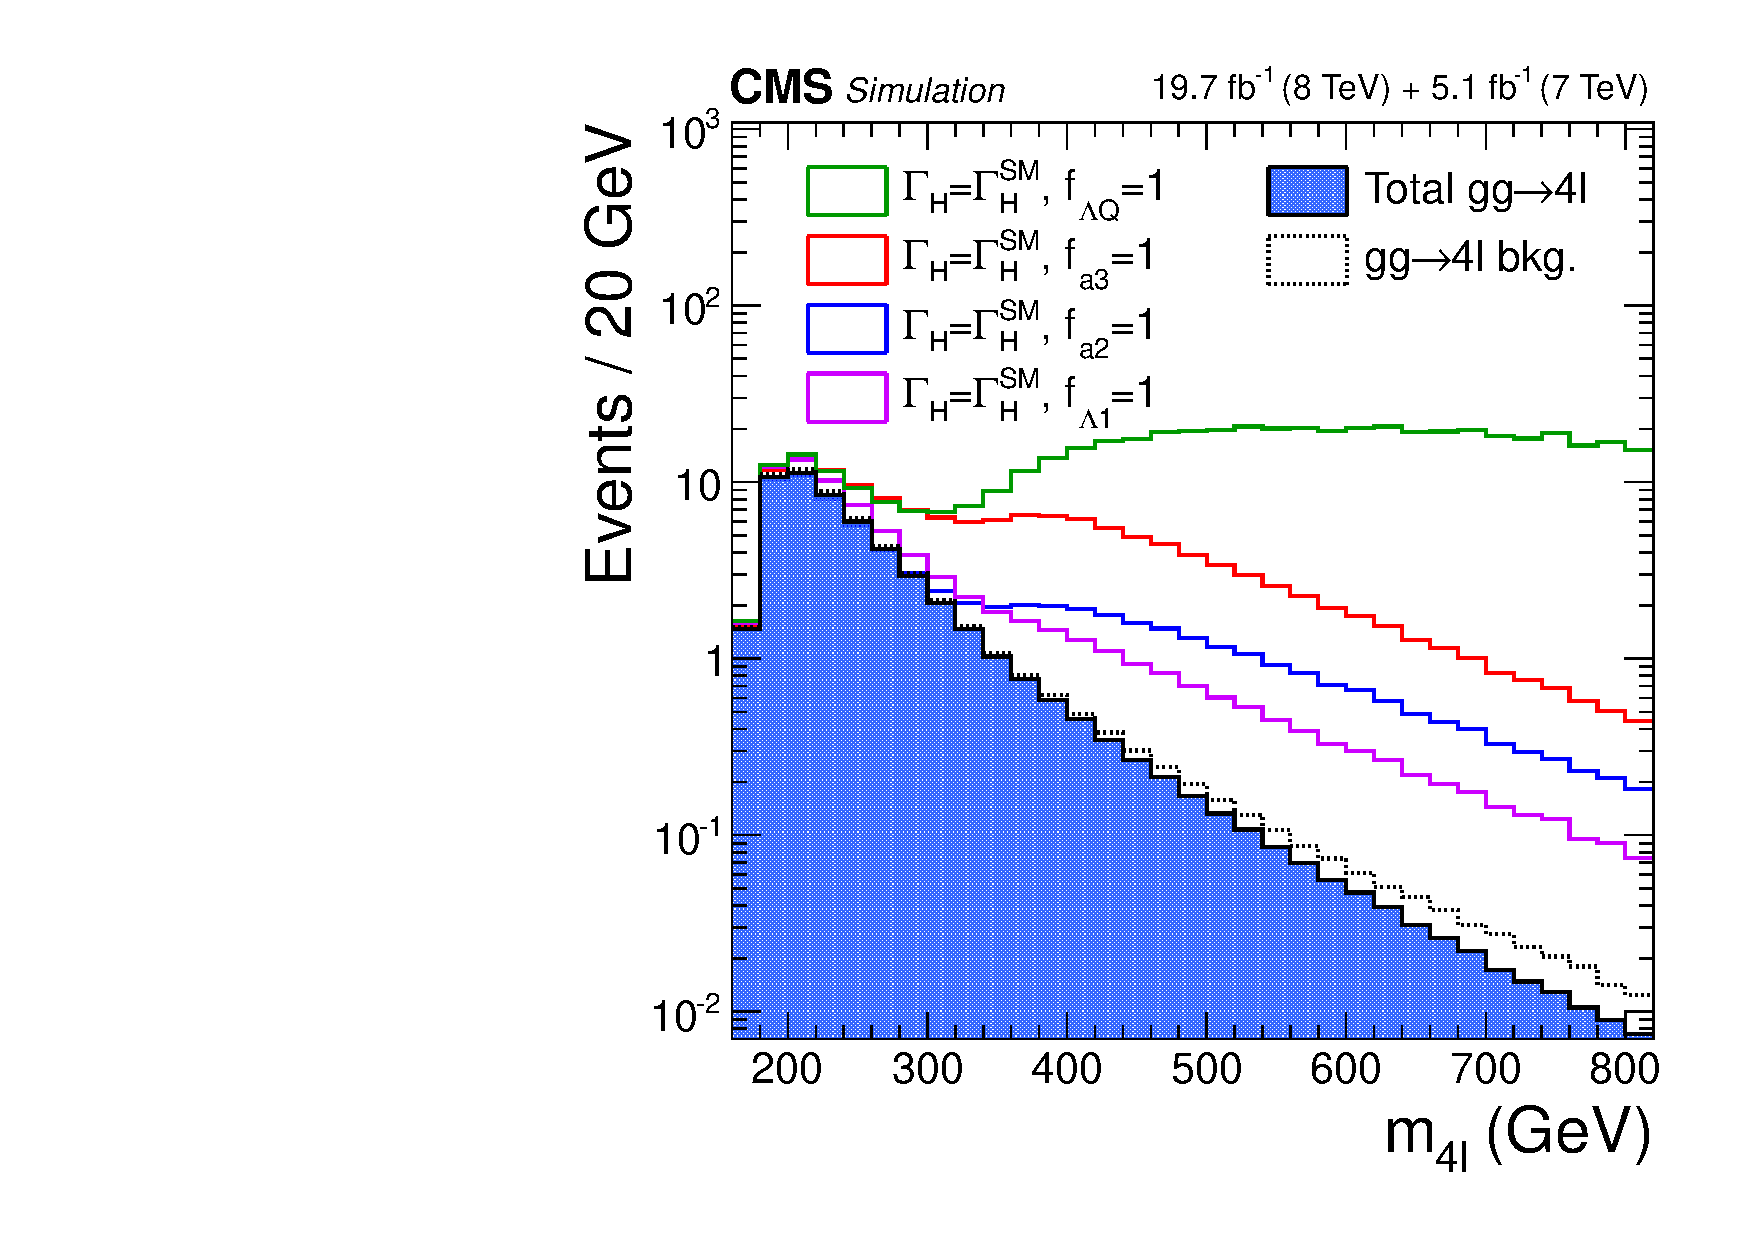
\includegraphics[width=0.45\linewidth]{Conclusion/cCanvas_MCFMBSM_GenLevel.pdf}
}
\caption[The $m_{4\ell}$ distributions in the off-shell region in the simulation of the $gg \to 4\ell$ process with the 
anomalous $\Lambda_{Q}$, $a_3$, $a_2$, and $\Lambda_{1}$ terms (open histograms) as well as the $a_1$  (SM filled histogram) term in decreasing order of enhancement at high $m_{4\ell}$.
In all cases, the background and its interference with the different signal hypotheses are included except in the case of the pure background (dashed black). The on-shell signal yield and the width $\Gamma_{H}$ are constrained to the SM expectations.]{ The $m_{4\ell}$ distributions in the off-shell region in the simulation of the $gg \to 4\ell$ process with the 
anomalous $\Lambda_{Q}$, $a_3$, $a_2$, and $\Lambda_{1}$ terms (open histograms) as well as the $a_1$  (SM filled histogram) term in decreasing order of enhancement at high $m_{4\ell}$.
In all cases, the background and its interference with the different signal hypotheses are included except in the case of the pure background (dashed black). The on-shell signal yield and the width $\Gamma_{H}$ are constrained to the SM expectations \cite{CMS_AN_2014_247}.
}
\label{fig:reweight_m4l_offshell}
\end{center}
\end{figure}


\section{$H \to VV \to 4\ell$ Spin/Parity Measurements}
\label{sec:Summary_SpinParity}

The interactions of a spin-zero, -one, or -two boson with
the SM particles is studied based on a scattering amplitude up to dimension five. A maximum likelihood fit of the signal and background distributions provides constraints on the anomalous couplings of the $H$ boson. The study focused on testing for the presence of anomalous effects in $HZZ$ interactions under spin-zero, -one, and -two hypotheses. The $HZ\gamma$ and $H\gamma\gamma$  interactions were probed using the $4\ell$ final state as well.

The exotic-spin study covers the analysis of mixed-parity spin-one states and ten spin-two hypotheses
under the assumption of production either via gluon fusion or quark-antiquark annihilation, or without
such an assumption. The spin-one hypotheses are excluded at a greater than 99.999\% C.L. while the spin-two boson with gravity-like minimal couplings is excluded at a 99.87\% C.L., and the other
spin-two hypotheses tested are excluded at a 99\% C.L. or higher.

Given the exclusion of the spin-one and spin-two scenarios,
constraints are set on the contribution of anomalous couplings to the
$HZZ$, $HZ\gamma$, and $H\gamma\gamma$ interactions
of a spin-zero $H$ boson, as summarized in table~\ref{tab:summary_spin0}.
Among these is the measurement of the $f_{a3}$ parameter,
which is defined as the fractional pseudoscalar cross section in the $H\to ZZ$ channel.
The constraint is $f_{a3}<0.43$ (0.40) at a 95\% C.L. for the positive (negative)
phase of the pseudoscalar coupling with respect to the dominant SM-like coupling
and $f_{a3}=1$ exclusion of a pure pseudoscalar hypothesis at a 99.98\% C.L..

All observations of the new particles spin/parity and tensor structure are consistent with the expectations for a scalar SM-like Higgs boson.

\subsection{Extensions}

We can perform a combination of the $H\to ZZ$ and $H \to WW$ measurements leading to tighter constraints on the $H$ boson spin-parity and anomalous $HVV$ interactions and higher exclusions of the spin-one and spin-two scenarios. Some of these combined results have already been presented in previous figures. For the $2_{m}^{+}$ hypothesis, in addition to the $H \to ZZ$ and $H \to WW$ final states combination with the $H \to \gamma\gamma$ final state is also helpful. A full summary of these results has been submitted for publication in \cite{Khachatryan:2014kca}. Figures \ref{fig:jp_summaryComb} and \ref{fig:hwwscans} give a few examples of these combinations.

\begin{figure}
  \centering
    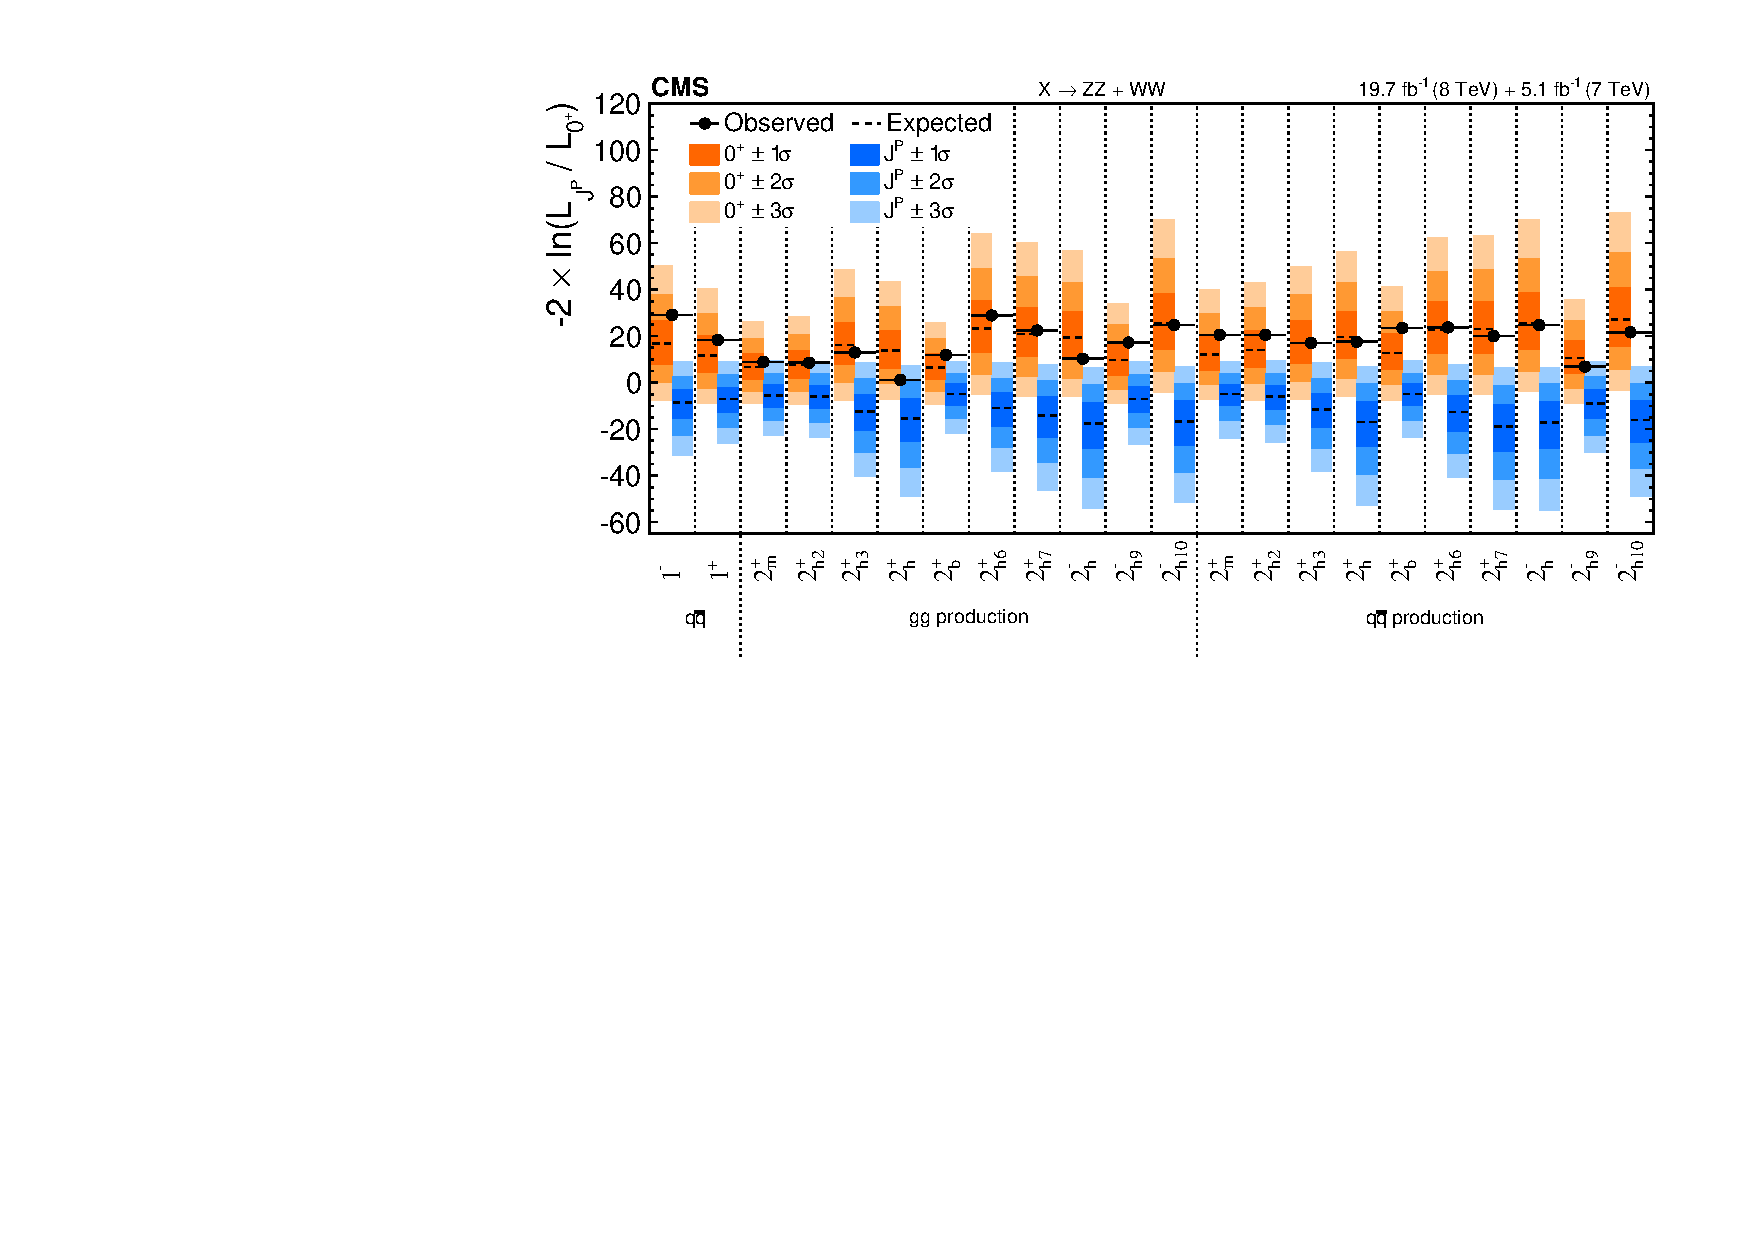
\includegraphics[width=0.9\textwidth]{Conclusion/JP_SummaryPlot_comb.pdf}
    \caption[Distributions of the test statistic $q=-2\ln(\mathcal{L}_{J^P}/\mathcal{L}_{0^+})$
       for the spin-one and spin-two $J^{P}$ models tested against the SM Higgs boson hypothesis
      in the combined $X\to ZZ$ and $WW$ analyses.
      The expected median and the 68.3\%, 95.4\%, and 99.7\% C.L. regions for the SM Higgs boson (orange, the left for each model)
      and for the alternative $J^P$ hypotheses (blue, right) are shown.
     The observed $q$ values are indicated by the black dots.]{
       Distributions of the test statistic $q=-2\ln(\mathcal{L}_{J^P}/\mathcal{L}_{0^+})$
       for the spin-one and spin-two $J^{P}$ models tested against the SM Higgs boson hypothesis
      in the combined $X\to ZZ$ and $WW$ analyses \cite{Khachatryan:2014kca}.
      The expected median and the 68.3\%, 95.4\%, and 99.7\% C.L. regions for the SM Higgs boson (orange, the left for each model)
      and for the alternative $J^P$ hypotheses (blue, right) are shown.
     The observed $q$ values are indicated by the black dots.
      \label{fig:jp_summaryComb}
      }

\end{figure}

\begin{figure}
  \centering
      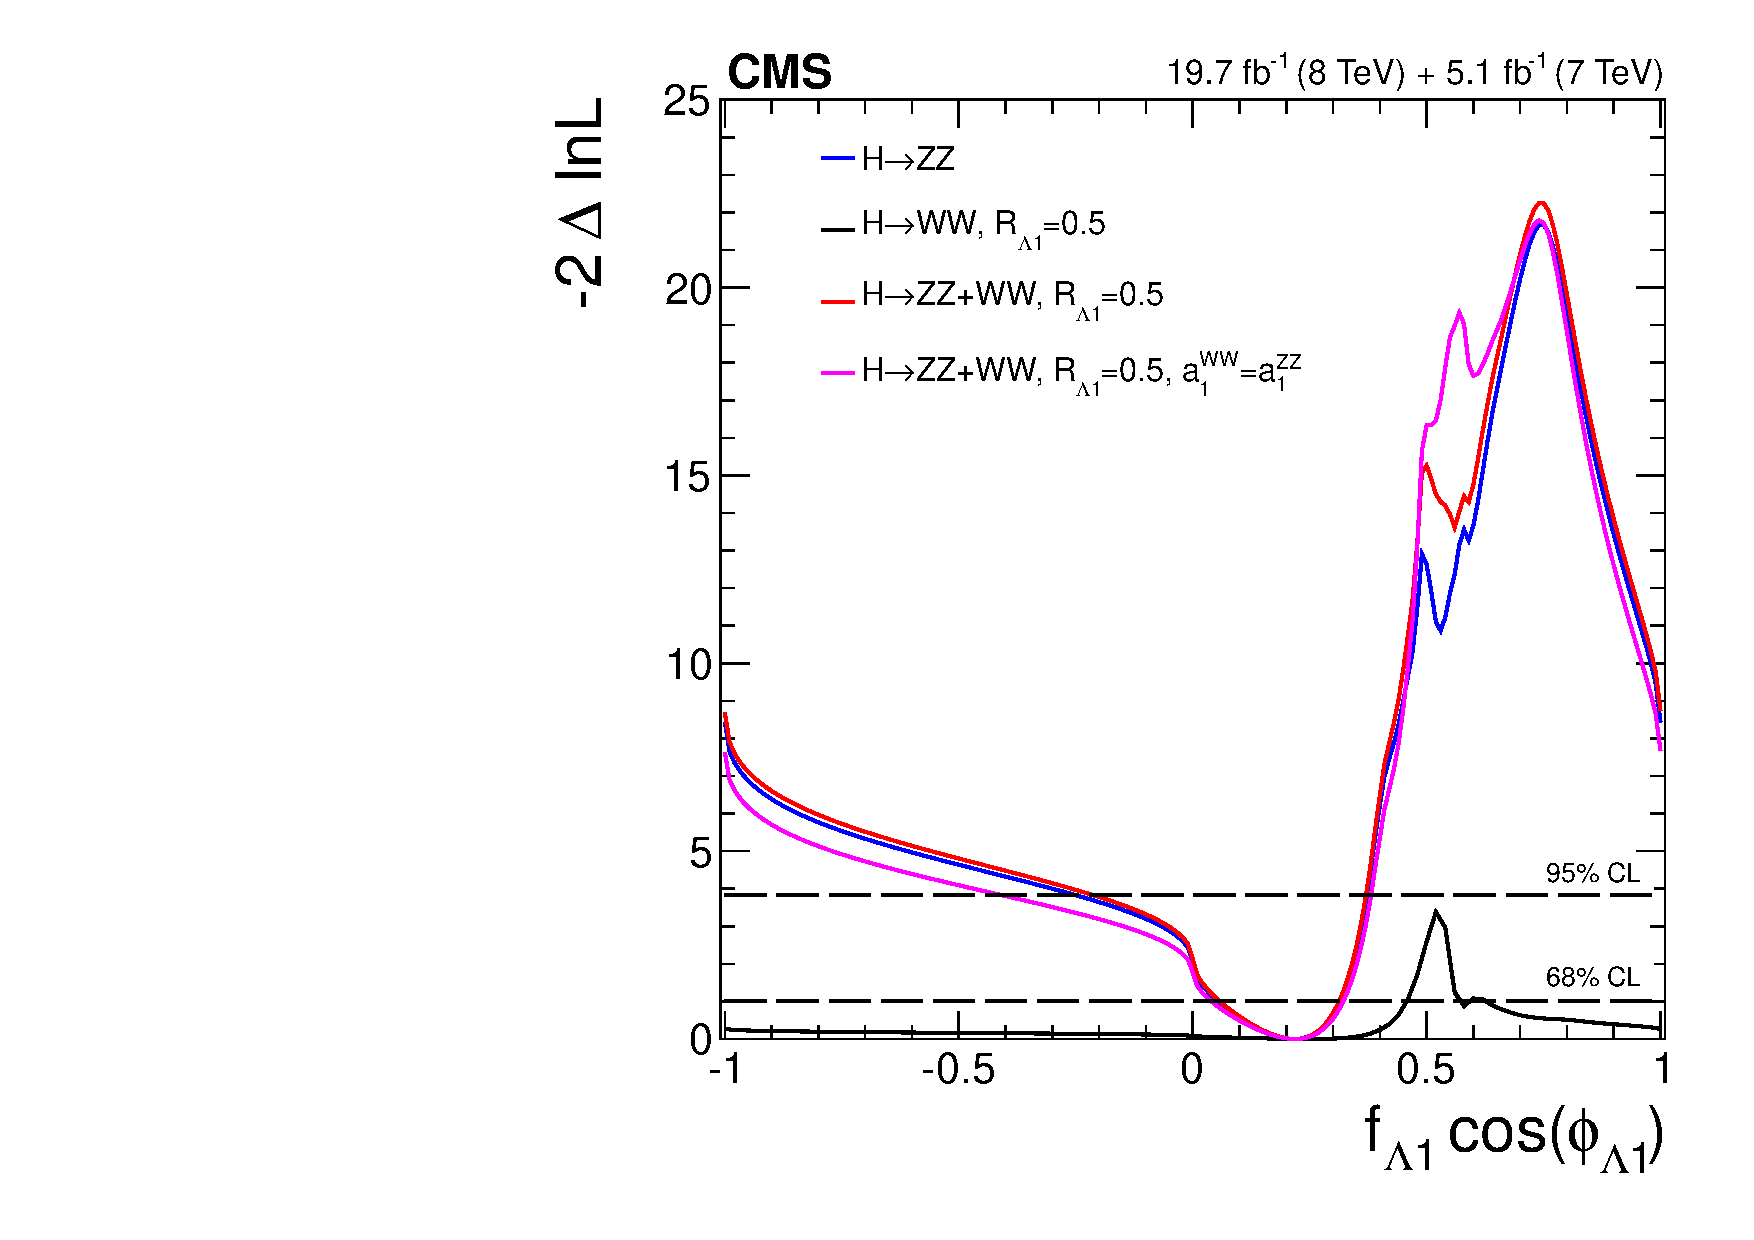
\includegraphics[width=0.32\textwidth]{Conclusion/flambda1_combine_ww.pdf}
      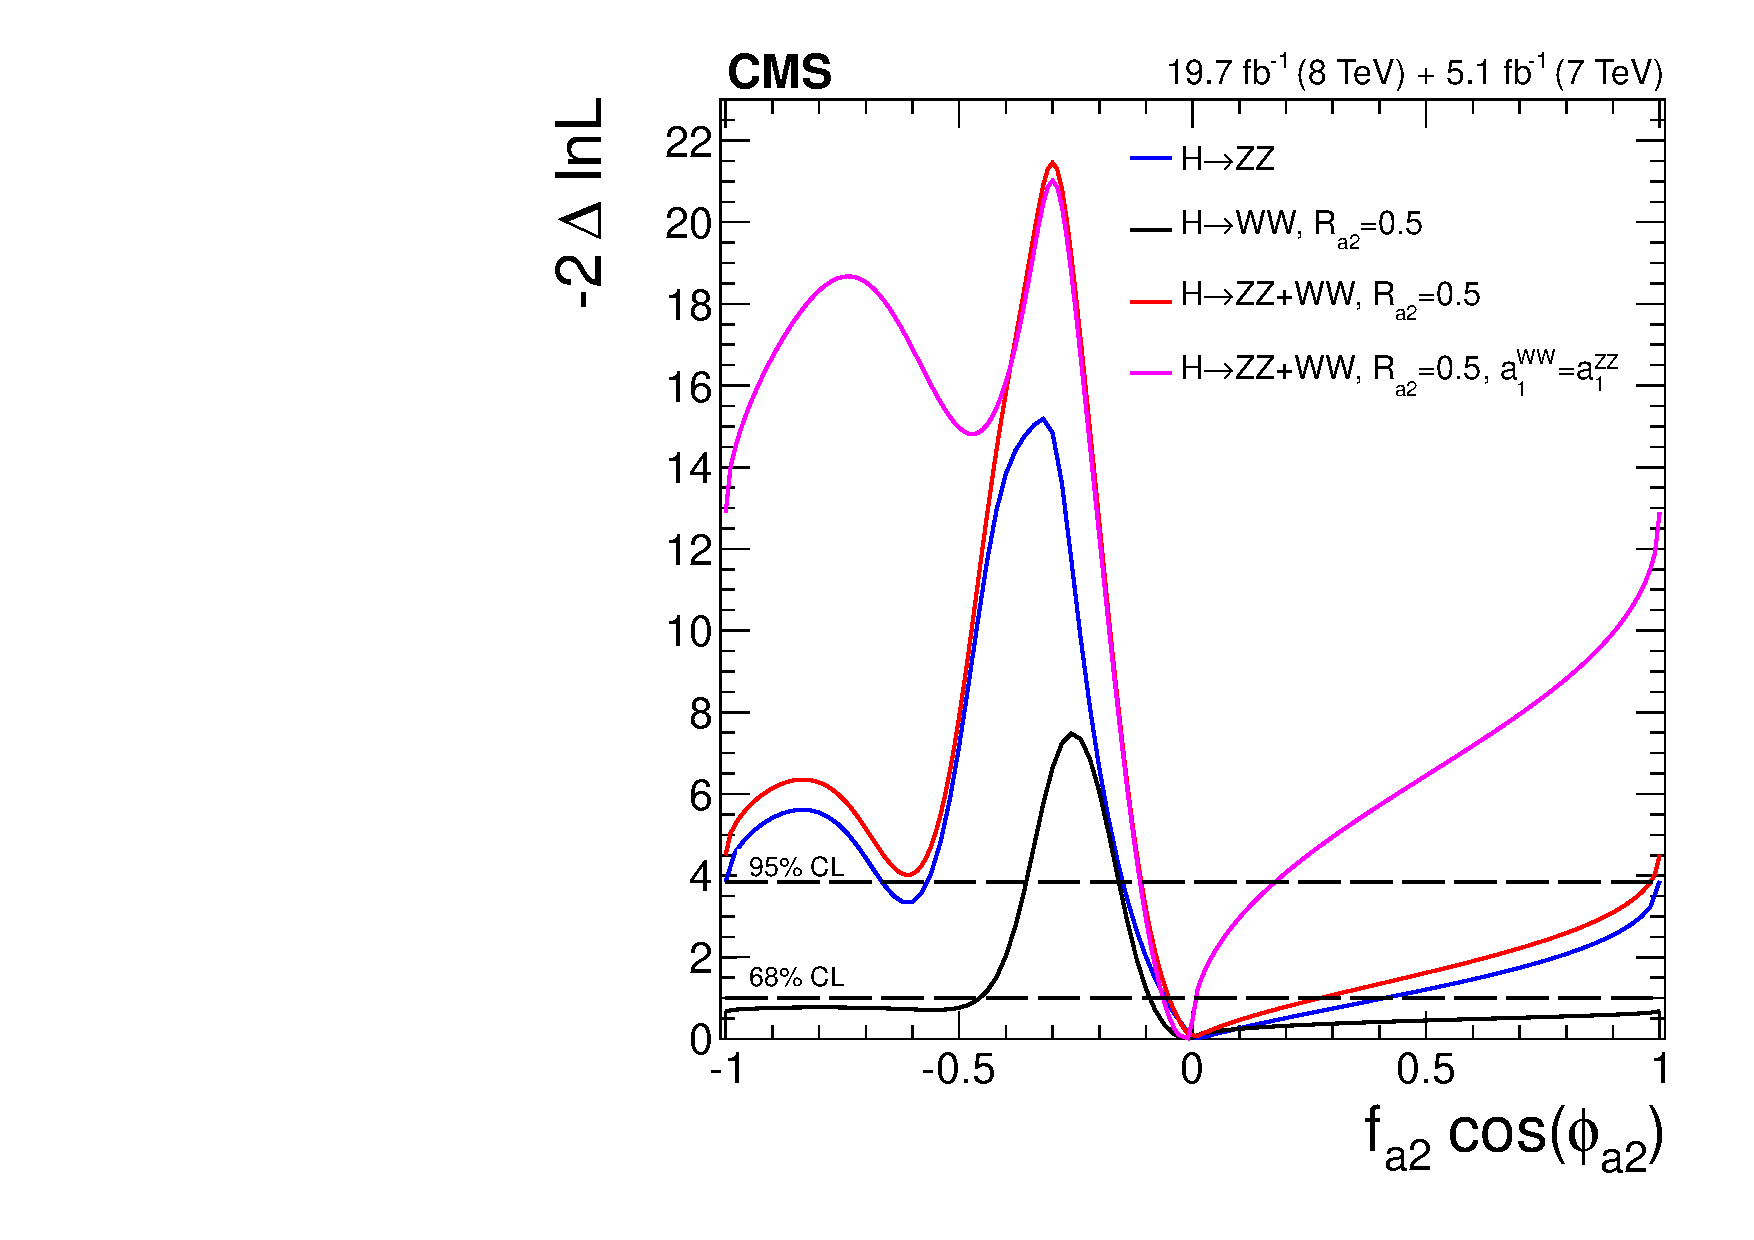
\includegraphics[width=0.32\textwidth]{Conclusion/fa2_combine_ww.pdf}
       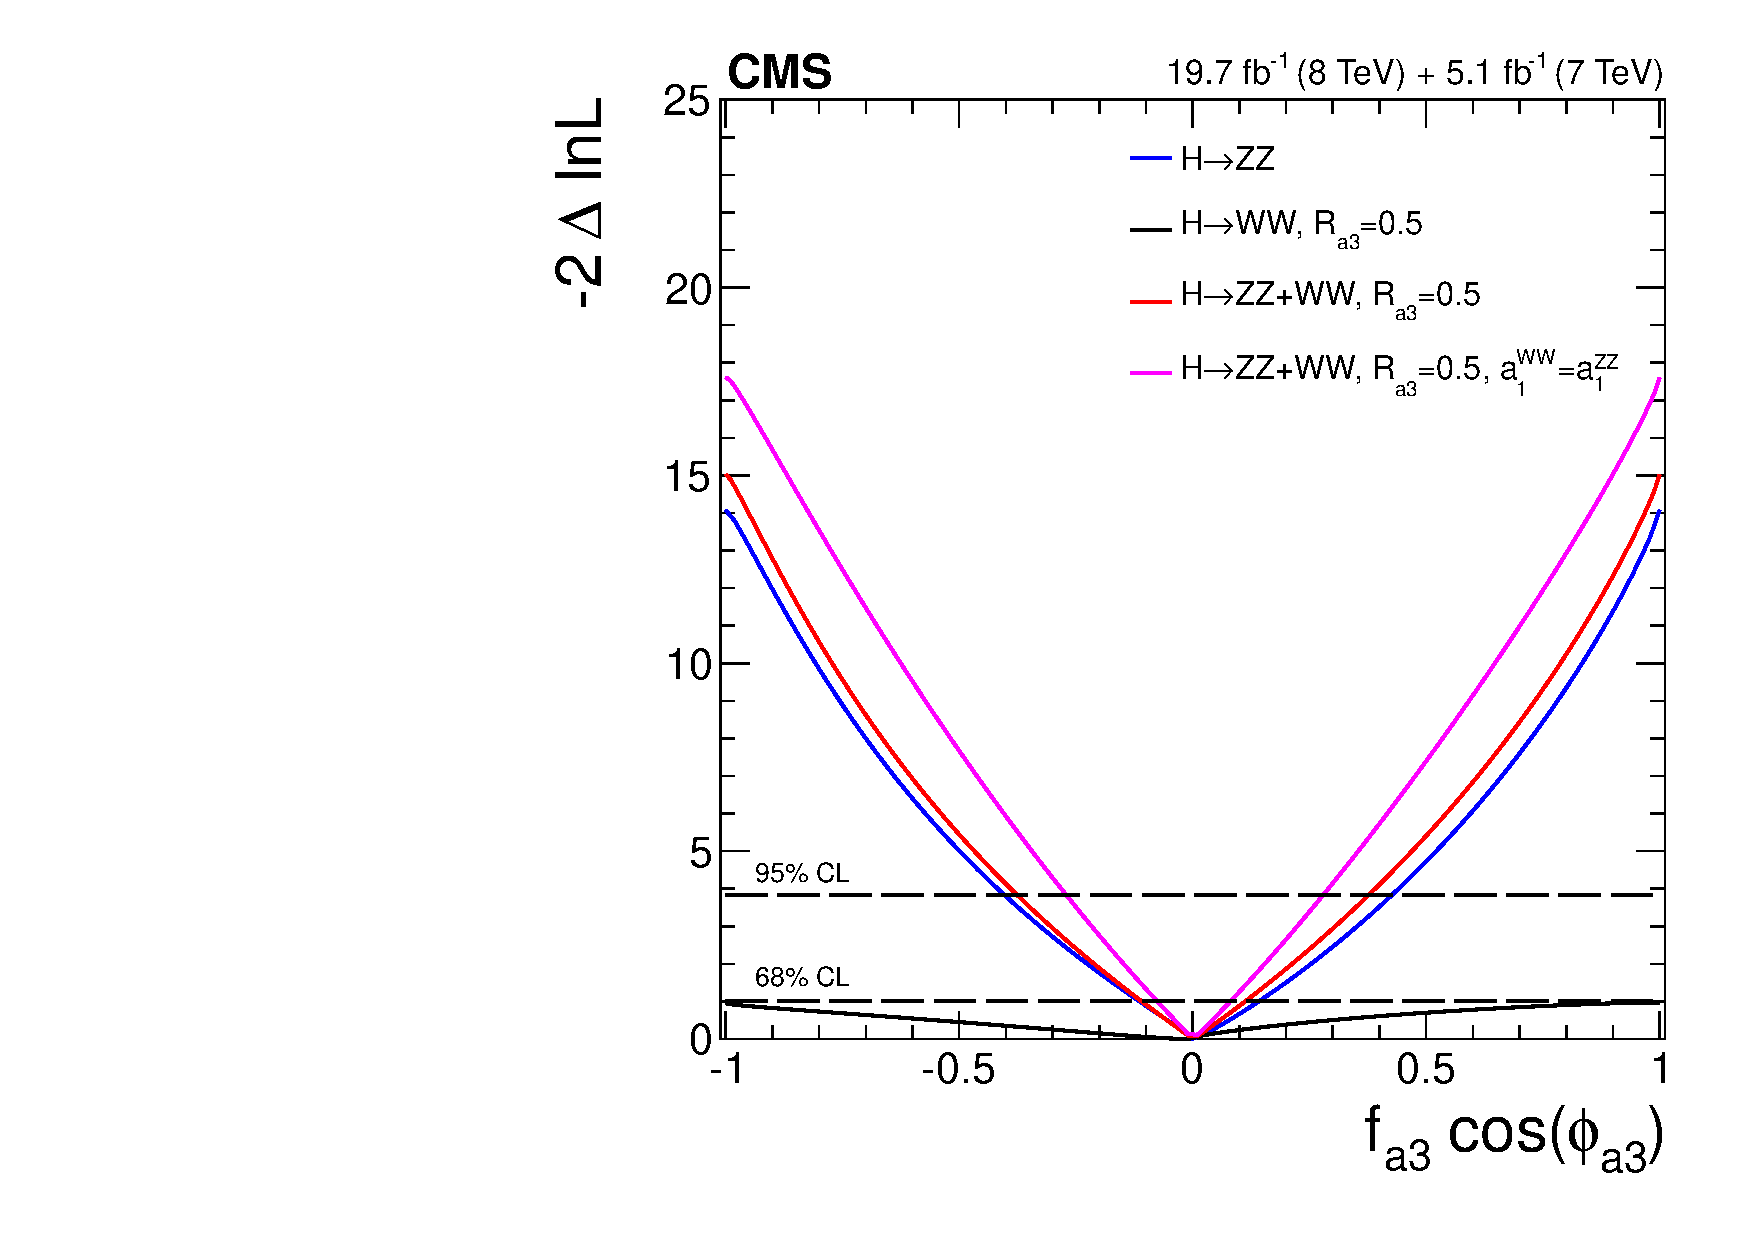
\includegraphics[width=0.32\textwidth]{Conclusion/fa3_combine_ww.pdf}
         \caption[Expected (dashed) and observed (solid) likelihood scans for effective fractions
	$f_{\Lambda1}$ (left), $f_{a2}$ (middle), $f_{a3}$ (right).
	The couplings studied are constrained to be real and all other anomalous couplings are fixed to the SM predictions.
	The $\cos\phi_{ai}$ term allows a signed quantity where $\cos\phi_{ai}=-1$ or $+1$.
	Plots show the combined  $H \to WW$ and $H \to ZZ$ results in terms of the $HZZ$ couplings for well motivated choices of the $WW$ and $ZZ$ coupling relationships.]{
         Expected (dashed) and observed (solid) likelihood scans for effective fractions
	$f_{\Lambda1}$ (left), $f_{a2}$ (middle), $f_{a3}$ (right).
	The couplings studied are constrained to be real and all other anomalous couplings are fixed to the SM predictions.
	The $\cos\phi_{ai}$ term allows a signed quantity where $\cos\phi_{ai}=-1$ or $+1$.
	Plots show the combined  $H \to WW$ and $H \to ZZ$ results in terms of the $HZZ$ couplings for well motivated choices of the $WW$ and $ZZ$ coupling relationships \cite{Khachatryan:2014kca}.
	}
    \label{fig:hwwscans}

\end{figure}

Additionally, this thesis work investigated the feasibility to measure anomalous $HVV$ couplings using either decay or production information in the future. These studies were not limited to high data LHC experiments but also investigated a future $e^{+}e^{-}$ collider as well. These studies looked at many different kinds of Higgs boson production and decay to project the ``ultimate" sensitivity of the MELA technique for these purposes. The results of these projection studies is shown in figure \ref{fig:fa3_project}, and additional studies in combining all information (production, decay, and off resonance production) are underway. 

\begin{figure}
  \centering
    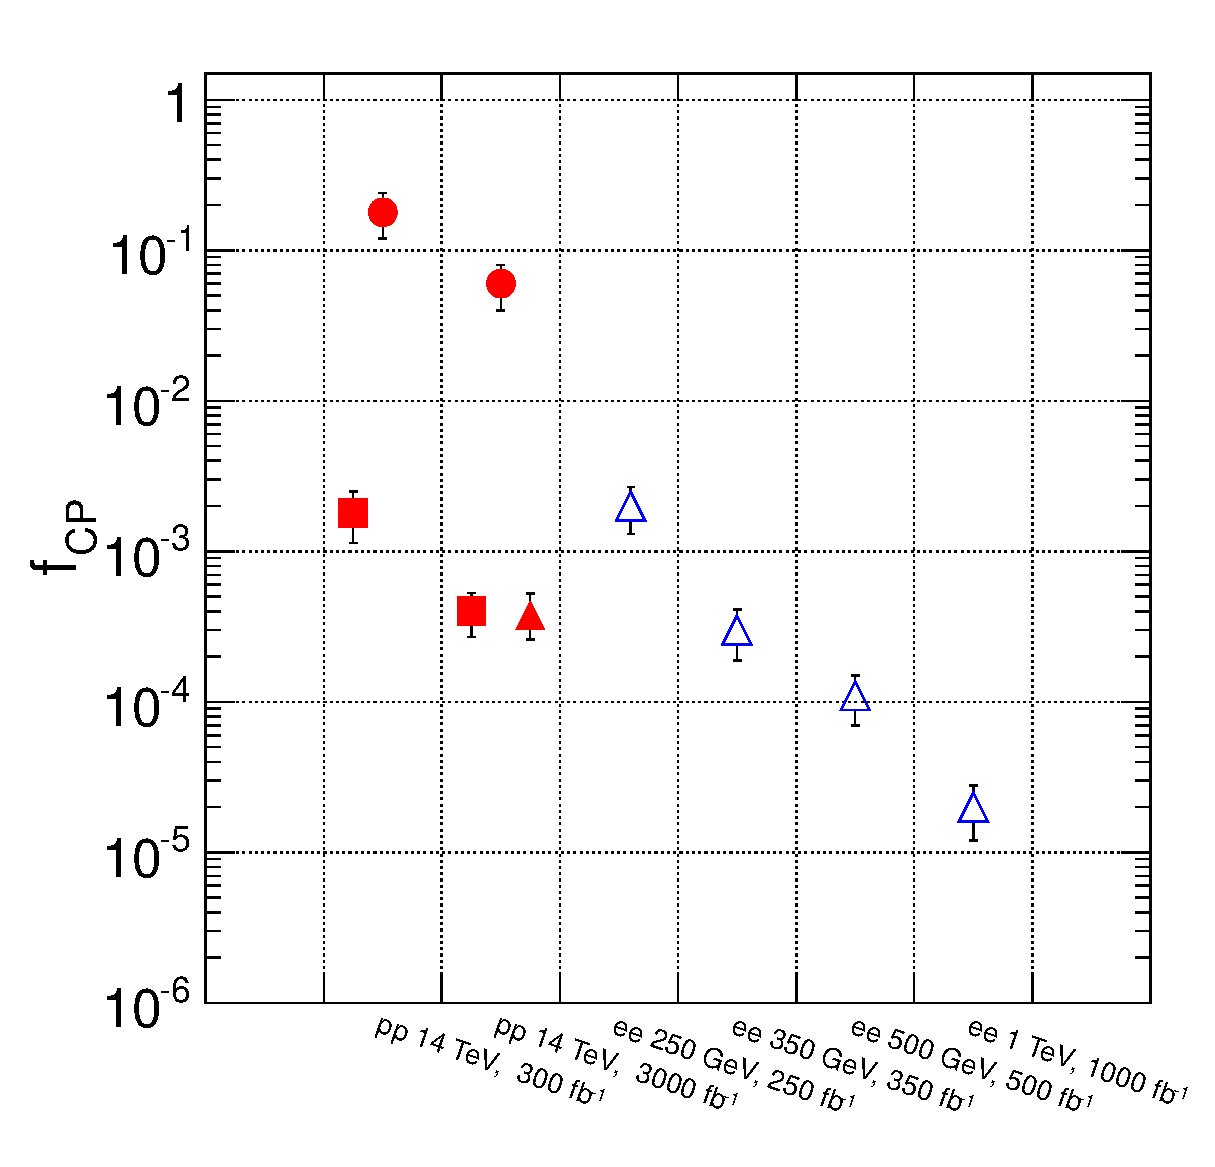
\includegraphics[width=0.45\textwidth]{Conclusion/summary_fcp.eps}
    \caption[Summary of precision in $f_{CP}$(generalization of $f_{a3}$) for $HVV$ couplings ($V = W, Z$) at the moment of $3\sigma$ measurement. Points indicate central values and error bars indicate $1\sigma$ deviations in the generated experiments modeling different luminosity scenarios at proton (solid red) or $e^{+}e^{-}$ (open blue) colliders. Measurements in three topologies $VH$ (triangles), $VBF$ (squares), and decay $H \to VV$ (circles) are shown.]{
       Summary of precision in $f_{CP}$(generalization of $f_{a3}$) for $HVV$ couplings ($V = W, Z$) at the moment of $3\sigma$ measurement. Points indicate central values and error bars indicate $1\sigma$ deviations in the generated experiments modeling different luminosity scenarios at proton (solid red) or $e^{+}e^{-}$ (open blue) colliders. Measurements in three topologies $VH$ (triangles), $VBF$ (squares), and decay $H \to VV$ (circles) are shown \cite{Anderson:2013afp}.
      \label{fig:fa3_project}
      }

\end{figure}

\section{Implications: Higgs boson as a tool}

Towards the beginning of this document a number of limitations to the SM were discussed. Beyond finding and understanding the Higgs boson, this work is an attempt to answer those questions. The information that we have gathered does not give complete answers to these questions, but does help focus the picture. In brief, this final discussion will present these questions again in the context of the answers that these studies have obtained.

The matter-antimatter asymmetry of the observable universe has been probed extensively with the spin/parity and tensor structure tests of the new boson. Specifically, the tests of $f_{a3}$ are designed to see if there is any $CP$-violating component to the observed resonance. To the current sensitivity of these measurements, no deviations from a pure $CP$-even state are observed. This does not rule out the observed boson as a source of significant $CP$-violation but the current data does not support it. Further, BSM models that postulate two Higgs bosons, one scalar (SM) and another pseudoscalar cannot be supported with the current data, because to a very high C.L. the observed boson is a scalar. Additionally, the search limits exclude additional bosons decaying to $VV$ up to $\sim\unit{1}{\TeV}$.

Offering a quantum explanation for gravity is also explicitly tested by the $CP$ studies presented in this work. Some of the spin-two models tested have motivations deeply connected to graviton hypotheses. Ten different spin-two models were tested against the SM hypothesis and in every one the data agrees with the SM hypothesis. Again, our data seems to point that the data we observe strongly favor the SM Higgs boson over any spin-two particle, and the exclusion of other bosons decaying to $VV$ up to $\sim\unit{1}{\TeV}$ disfavor BSM particles up to this mass scale.

The potential connection between the observed Higgs boson and dark matter is tested by almost every measurement presented in this thesis. If there was a significant branching fraction of the observed boson to dark matter the production mechanism could show a deviation from SM behavior. Additionally, a significant Higgs boson -- dark matter coupling would produce an increased total width of the Higgs boson that could be observed in the off shell width measurements. Finally, if any of the $HVV$ coupling measurements were to show a deviation from the SM predictions it could be a sign of a dark matter particle increasing the contribution of that particular coupling. Given that all observations are currently consistent with the SM Higgs boson, dark matter still remains one of the most interesting mysteries in the universe.

The hierarchy problem actually becomes more confusing given current observations. The mass of observed Higgs boson is observed to be very low compared to most theoretical predictions making the `parameter tuning' that lies behind the hierarchy problem more strange.

Overall this thesis work presents some of the most comprehensive search and characterization studies of the new Higgs boson that have been undertaken. The LHC accelerator and CMS experiment should be congratulated for their wonderful performance leading to these studies. While many questions about the SM remain, all signs point to the observed boson being consistent with one that would arise from the Higgs mechanism, offering the solution to at least one question.